\def\HandoutMode{handout}
\def\ButtonsMode{0}
\documentclass[\HandoutMode,table]{beamer}

\mode<presentation>
\usetheme{CambridgeUS}
\usecolortheme{seahorse}

\usepackage[english]{babel}
\usepackage[utf8]{inputenc}
\usepackage[T1]{fontenc}
\usepackage{xspace}
\usepackage[noend]{algorithm2e}
\usepackage{listings}
\usepackage{graphicx}
\usepackage{tikz}
\usepackage{ifthen,xstring,calc,pgfopts,tikz-uml}
\usepackage{xcolor}
\usepackage{booktabs}
\usepackage{subfig}
\usepackage[justification=centering,format=hang]{caption}
\usepackage{adjustbox}

\ifthenelse{\equal{\HandoutMode}{handout}}{%
    \usepackage{pgfpages}
    \pgfpagesuselayout{2 on 1}[a4paper,border shrink=5mm]
}{}

\newcommand{\myTitle}{Uberfuzz\xspace}
\newcommand{\mySubtitle}{A Cooperative Fuzzing Framework\xspace}
\newcommand{\myDegree}{Master of Science in Artificial Intelligence\xspace}
\newcommand{\myName}{Andrea Jemmett\xspace}
\newcommand{\myProf}{Dr. Sanjay Rawat\xspace}
\newcommand{\myOtherProf}{Put name here\xspace}
\newcommand{\mySupervisor}{Put name here\xspace}
\newcommand{\myFaculty}{Faculty of Science\xspace}
\newcommand{\myDepartment}{Dept.\ of Computer Science\xspace}
\newcommand{\myUni}{Vrije Universiteit Amsterdam\xspace}
\newcommand{\myLocation}{Amsterdam, Netherlands\xspace}
\newcommand{\myTime}{August 2019\xspace}

\newcommand{\eg}{e.\,g.}
\newcommand{\Eg}{E.\,g.}
\newcommand{\ie}{i.\,e.}

\newcommand\hicell{\cellcolor[gray]{.85}}

\newcommand\djpeg{\texttt{djpeg}}
\newcommand\objdump{\texttt{objdump}}
\newcommand\tiffpdf{\texttt{tiff2pdf}}
\newcommand\listswf{\texttt{listswf}}

\newcounter{lipsumi}
\newcommand\lipsumseqrestart{\setcounter{lipsumi}{1}}
\lipsumseqrestart%
\newcommand\lipsumi{\value{lipsumi}}
\newcommand\lipsumseq[1][1]{%
    \lipsum[\lipsumi-\the\numexpr\lipsumi+#1-1]
    \addtocounter{lipsumi}{#1}
}

\newcommand\sut{\ac{SUT}}
\newcommand\afl{AFL}
\newcommand\aflfast{AFLFast}
\newcommand\fairfuzz{FairFuzz}
\newcommand\honggfuzz{Honggfuzz}
\newcommand\vuzzer{VUzzer}


\newcommand\ac[1]{#1}           % dummy \ac command, does nothing
\renewcommand\hicell{\cellcolor[RGB]{255, 101, 66}}
\newcommand\figwidth\textwidth
\newcommand\buttons[1]{\if\ButtonsMode1 #1 \fi}

\title{\myTitle}
\subtitle{\mySubtitle}
\author{\myName}
\institute[VU]{\myUni}

\AtBeginSubsection[]
{%
    \begin{frame}
        \tableofcontents[currentsection,currentsubsection]
    \end{frame}
}

\lstdefinelanguage[modern]{C}[ANSI]{C}{%
    morekeywords={bool,true,false,size_t,uint8_t}}

\lstdefinestyle{mystyle}{%
    basicstyle=\small\ttfamily,
    keywordstyle=\color{blue},
    stringstyle=\color{teal},
    commentstyle=\color{red}}

\lstdefinestyle{nonumbered}{%
    style=mystyle,
    numbers=none}

\lstdefinestyle{numbered}{%
    style=mystyle,
    numbers=left,
    numbersep=12pt,
    numberstyle=\tiny,
    xleftmargin=12pt}

\begin{document}

\frame{\titlepage}

\begin{frame}{Outline}
    \tableofcontents[pausesections]
\end{frame}

\section{Background and Related Work}

\subsection{Fuzzing Techniques}

\begin{frame}{Fuzzing}
    \begin{itemize}
        \item<1-> term coined in 1988 during a quiet and stormy night\ldots\
        \item<2-> established reliability and security testing practice
        \item<2-> ``Mayhem'' wins 2016 DARPA Cyber Grand Challenge
        \item<2-> used in industry by Microsoft and Google
    \end{itemize}
\end{frame}

\begin{frame}[fragile]{Challenges}
\begin{lstlisting}[language={[modern]C},style=numbered]
void process_buffer (const char *buf) {
    size_t n = strlen(buf);
    if (n > 1000 || n < 4)
        return;
    if (buf[1] == 0xFF && buf[0] == 0xFD) {
        uint8_t i = (uint8_t) buf[3];
        if (i > 3 && i < n) {
            if (strncmp(&buf[i], "CHK", 3) == 0) {
                // bug here
            }
        }
    }
}
\end{lstlisting}
\end{frame}

\begin{frame}{Black Box Mutational Fuzzing}
    \begin{block}<+->{General operation}
        \setbeamercovered{transparent}
        \begin{enumerate}[<+->]
            \item{} select input from seed corpus
            \item{} mutate input to produce new one
            \item{} execute SUT with mutated input
            \item{} monitor for unexpected behaviours
        \end{enumerate}
    \end{block}
    \begin{exampleblock}<+->{Examples}
        \begin{itemize}
            \item{} Radamsa, zzuf
            \item{} Basic Fuzzing Framework
        \end{itemize}
    \end{exampleblock}
\end{frame}

\begin{frame}{Coverage-Based Gray Box Fuzzing}
    \begin{block}<+->{Overview}
        \begin{itemize}
            \item{} execution is monitored to gain \alert{feedback}
            \item{} the feedback is used to better instruct the search
        \end{itemize}
    \end{block}
    \begin{exampleblock}<+->{American Fuzzy Lop}
        \begin{itemize}
            \item{} instruments the SUT to get coverage feedback
            \item{} selects ``favorite'' inputs more often
            \item{} mutation as deterministic and havoc stages
            \item{} stores generated input if branch hit counts change bucket
        \end{itemize}
    \end{exampleblock}
\end{frame}

\begin{frame}<presentation:0>[noframenumbering]{Other Gray Box Fuzzers}
    \setbeamercovered{transparent}
    \begin{description}
        \item[AFLFast]<1>
            \begin{itemize}
                \item{} models fuzzing as Markov chain
                \item{} focus fuzzing on low frequency paths
            \end{itemize}
        \item[FairFuzz]<2>
            \begin{itemize}
                \item{} focus fuzzing on rare branches
                \item{} search strategy prioritizes inputs that hit a rare branch
                \item{} mutation preserves parts necessary to hit rare branch
            \end{itemize}
        \item[Honggfuzz]<3>
            \begin{itemize}
                \item{} simplifies operation
                \item{} uses hardware sources for coverage
            \end{itemize}
        \item[VUzzer]<4>
            \begin{itemize}
                \item{} population-based model (\ie~Evolutionary Algorithms)
                \item{} fitness function uses branch hit frequencies
                \item{} application-aware recombination and mutation operators
            \end{itemize}
    \end{description}
\end{frame}

\begin{frame}{Symbolic-Assisted White Box Fuzzing}
    \begin{block}{Key features}
        \begin{itemize}
            \item{} uses symbolic execution to collect path constraints
            \item{} constraints are solved to provide new inputs
            \item<alert@2-> constraints not always solvable or solver is slow
        \end{itemize}
    \end{block}
    \begin{exampleblock}<3->{Examples}
        \begin{itemize}
            \item{} DART and SAGE
            \item{} EXE and KLEE
            \item{} Mayhem
        \end{itemize}
    \end{exampleblock}
\end{frame}

\subsection{Hybrid and Cooperative Fuzzing}

\begin{frame}{Hybrid Approaches}
    \structure<+->{Merge white box fuzzers with black or gray box ones}
    \\~\\
    \begin{exampleblock}<+->{Driller}
        \begin{itemize}
            \item{} uses AFL and custom symbolic execution engine
            \item{} AFL becomes ``stuck'' $\rightarrow$ s.e.\ generates new inputs
        \end{itemize}
    \end{exampleblock}
\end{frame}

\begin{frame}{Cooperative Fuzzing}
    \begin{block}<+->{A system that allows fuzzers to share information to achieve a common goal}
        \begin{itemize}
            \item{} fuzzing is non-deterministic
            \item{} there is no best fuzzer for all possible programs
            \item{} information sharing as a mean to share features
                \note{example: VUzzer may share input with magic bytes to AFL}
        \end{itemize}
    \end{block}
    \begin{exampleblock}<+->{Examples}
        \begin{itemize}
            \item{} Levy Flights over an input space
            \item{} Chemotactic test case recombination
        \end{itemize}
    \end{exampleblock}
\end{frame}

\section{Cooperative Fuzzing Framework}

\subsection{System Design}

\begin{frame}{Common Fuzzer Interface}
    \begin{block}{Three API primitives}
        \begin{itemize}[<+->]
            \item{} \alert{extract} test cases from fuzzer
            \item{} \alert{inject} test cases into fuzzer
            \item{} \alert{congestion control} for slower or generational
                fuzzers
        \end{itemize}
    \end{block}
\end{frame}

\begin{frame}{Central Decisional Unit}
    \begin{columns}
        \begin{column}{.5\textwidth}
            \begin{figure}
                \includegraphics[width=.5\textwidth]{figures/dia/system_design_logical}
                \caption{Logical view}
            \end{figure}
            \begin{figure}
                \includegraphics[width=.5\textwidth]{figures/dia/system_design_physical}
                \caption{Physical view}
            \end{figure}
        \end{column}
        \begin{column}{.5\textwidth}
            \begin{itemize}
                \item{} acts as intermediary for information exchange
                \item{} uses API to implement a strategy
            \end{itemize}
        \end{column}
    \end{columns}
\end{frame}

\begin{frame}[fragile]{Cooperative Fuzzing Strategies}
\scalebox{.8}{%
    \begin{algorithm}[H]
        \DontPrintSemicolon%
        \SetKwFunction{Score}{Score}
        \SetKwFunction{Winning}{Winning}
        \SetKwFunction{Inject}{Inject}
        \SetKwFunction{WinningC}{WinningCongestion}
        % \SetKwInOut{Input}{Input}\SetKwInOut{Output}{Output}
        % \Input{Set of running fuzzers $F$. Set of fuzzers that need congestion control $F_c$}
        % \BlankLine%
        \ForEach{$f \in F_c$}{%
            $W_f \leftarrow \emptyset$\;
        }
        \While{all fuzzers are running}{%
            \If{new test-case $t$ from a fuzzer $f_t$}{%
                $S \leftarrow \emptyset$\;
                \ForEach{$f \in F \setminus \{f_t\}$}{%
                    $s \leftarrow \Score{f, t}$\;
                    \uIf{$f \in F_c$}{%
                        $W_f \leftarrow W_f \cup \{(t, s)\}$\;
                    }
                    \Else{%
                        $S \leftarrow S \cup \{(f, s)\}$\;
                    }
                }
                \ForEach{$f \in \Winning{S}$}{%
                    \Inject{f, t}\;
                }
            }
            \ForEach{$f \in F_c$}{%
                \If{$f$ is ready to receive inputs}{%
                    \ForEach{$t \in \WinningC{$W_f$}$}{%
                        \Inject{f, t}\;
                    }
                    $W_f \leftarrow \emptyset$\;
                }
            }
        }
    \end{algorithm}
}
\end{frame}

\subsection{System Implementation}

\begin{frame}{Overview}
    \begin{tikzpicture}
        \umlbasiccomponent[x=-2,y=0]{Fuzzer}
        \begin{umlcomponent}[x=3,y=0]{CFF}
            \umlbasiccomponent[x=0,y=0]{Driver}
            \umlbasiccomponent[x=4,y=1.5]{Master}
            \only<3->{%
                \umlassemblyconnector[interface=Interesting,geometry=-|,%
                    anchors=180 and 90,first arm]{Master}{Driver}
            }
            \only<4->{%
                \umlassemblyconnector[interface=Metric,geometry=|-,%
                    anchors=230 and 10]{Master}{Driver}
            }
            \only<5->{%
                \umlassemblyconnector[interface=Inject,geometry=-|,%
                    anchors=-30 and 290,first arm]{Driver}{Master}
            }
        \end{umlcomponent}
        \only<2->{%
            \umlassemblyconnector[interface=API]{Driver}{Fuzzer}
        }
    \end{tikzpicture}
\end{frame}

\section{Evaluation}

\subsection{Single Fuzzers Evaluation}

\begin{frame}{Finding the Best Fuzzer}
    \begin{block}{Choice of fuzzers}
        \begin{description}
            \item[\aflfast] CGF with focus on paths
            \item[\fairfuzz] CGF with focus on branches
            \item[\honggfuzz] hardware feedback, high throughput
            \item[\vuzzer] application-aware, population-based
        \end{description}
    \end{block}
    \begin{block}{Experiment design}
        \begin{enumerate}
            \item{} run each fuzzer independently for 24 hours
            \item{} collect coverage with granularity 1 minute
            \item{} compare mean coverage over 5 runs
        \end{enumerate}
    \end{block}
\end{frame}

\begin{frame}{Mean Coverage}
    \begin{table}
        \scriptsize
        \begin{tabular}{l*{4}c}
            \textbf{\sut} & \textbf{\aflfast} & \textbf{\fairfuzz} &
    \textbf{\honggfuzz} & \textbf{\vuzzer} \\
\bottomrule%
\djpeg& $3739.4 \pm 113.831$ & $4043.2 \pm 103.838$ &
    \hicell$4112.8 \pm 39.5483$ & $2801 \pm 53.5514$ \\
\objdump& $4762.6 \pm 23.3693$ & \hicell$5067 \pm 62.6832$ &
    $4132.4 \pm 104.8$ & $3162.2 \pm 138.462$ \\
\tiffpdf& \hicell$8971.2 \pm 152.865$ & $8813.8 \pm 146.756$ &
    $5260.2 \pm 148.591$ & $3616 \pm 34.6427$ \\
\listswf& $6831.6 \pm 2615.24$ & \hicell$8586.8 \pm 87.7467$ &
    $6345.6 \pm 2358.52$ & $5048.2 \pm 90.3928$


        \end{tabular}
    \end{table}
\end{frame}

\begin{frame}{Bayesian Estimation of Means}
    \renewcommand\figwidth{.33\textwidth}
    \setcounter{subfigure}{0}
    \begin{figure}
        \subfloat[\djpeg\\\honggfuzz\ vs.\ \fairfuzz]{%
            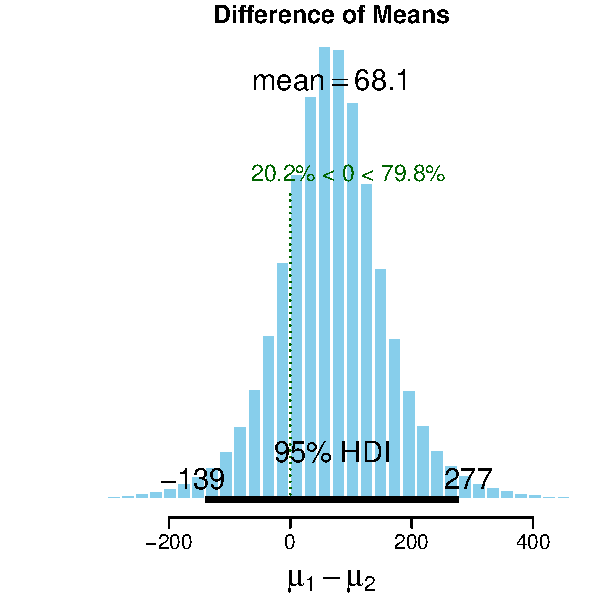
\includegraphics[width=\figwidth]{figures/cropped/djpeg-m-hongg-fair}
        }
        \subfloat[\objdump\\\fairfuzz\ vs.\ \aflfast]{%
            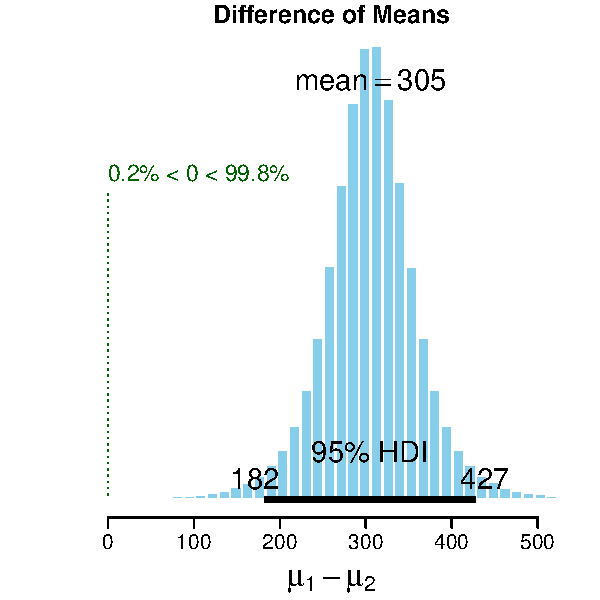
\includegraphics[width=\figwidth]{figures/cropped/objdump-m-fair-afl}
        }
        \subfloat[\tiffpdf\\\aflfast\ vs.\ \fairfuzz]{%
            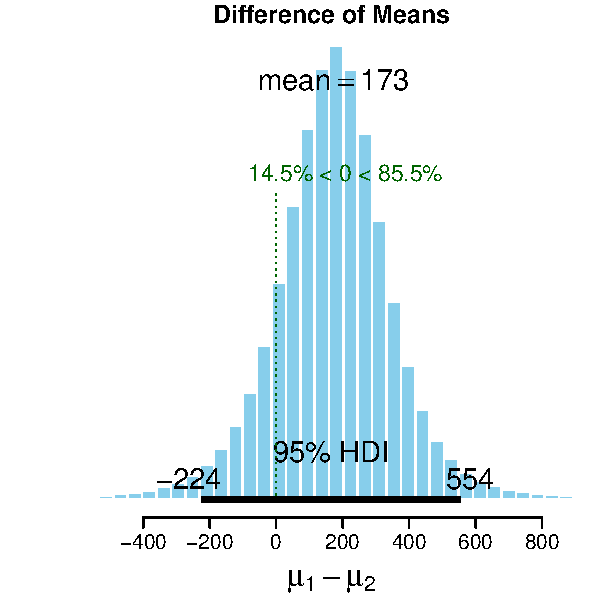
\includegraphics[width=\figwidth]{figures/cropped/tiff2pdf-m-afl-fair}
        }
    \end{figure}
\end{frame}

\begin{frame}{Fuzzers Uncover Disjoint Transitions Sets}
    \begin{table}
        \begin{tabular}{l c l c}
            \textbf{\sut} & \multicolumn{2}{c}{\textbf{best single}} & \textbf{union} \\
\bottomrule%
\djpeg& $4112.8 \pm 39.5476$ & \honggfuzz& \hicell$4157.2 \pm 40.0495$ \\
\objdump& $5067 \pm 62.6821$ & \fairfuzz& \hicell$5404.6 \pm 38.1997$ \\
\tiffpdf& $8971.2 \pm 152.8626$ & \aflfast& \hicell$9695 \pm 129.7239$ \\
\listswf& $8586.8 \pm 87.7451$ & \fairfuzz& \hicell$8916.6 \pm 83.8365$


        \end{tabular}
    \end{table}
    \vspace{2\baselineskip}
    \structure{Bayesian estimation agrees, except for \djpeg}
\end{frame}

\subsection{Cooperative Fuzzing Evaluation}

\begin{frame}{Evaluating the Effect of Cooperation}
    \begin{block}{Cooperative strategies}
        \begin{itemize}
            \item{} score is number of newly discovered BTS transitions
            \item{} single highest winner strategy
            \item{} multiple positive-scored winners strategy
        \end{itemize}
    \end{block}
    \begin{block}{Experiment design}
        \begin{enumerate}
            \item{} run CFF with selected strategy for 6 hours
            \item{} drivers log coverage for respective fuzzer
            \item{} compare mean coverage over 5 runs against union of fuzzers
        \end{enumerate}
    \end{block}
\end{frame}

\begin{frame}{Mean Coverage}
    \begin{table}
        \begin{tabular}{l c c c}
            \textbf{\sut} & \textbf{multi} & \textbf{single} & \textbf{union} \\
\bottomrule%
\djpeg& $4056.4 \pm 76.9499$ & \hicell$4078.4 \pm 85.6738$ & $4028.6 \pm 47.7396$ \\
\objdump& $5414.6 \pm 224.121$ & \hicell$5529.6 \pm 338.651$ & $5035.6 \pm 54.5944$ \\
\tiffpdf& \hicell$8765.6 \pm 183.682$ & $8577.6 \pm 99.2457$ & $8623.2 \pm 183.399$ \\
\listswf& \hicell$9008.4 \pm 122.81$ & $8801.4 \pm 96.4045$ & $8916.6 \pm 83.8381$


        \end{tabular}
    \end{table}
\end{frame}

\begin{frame}{Bayesian Estimation of Means}
    \renewcommand\figwidth{.28\textwidth}
    \setcounter{subfigure}{0}
    \begin{figure}
        \begin{adjustbox}{center}
            \subfloat[\djpeg\\single vs.\ union]{%
                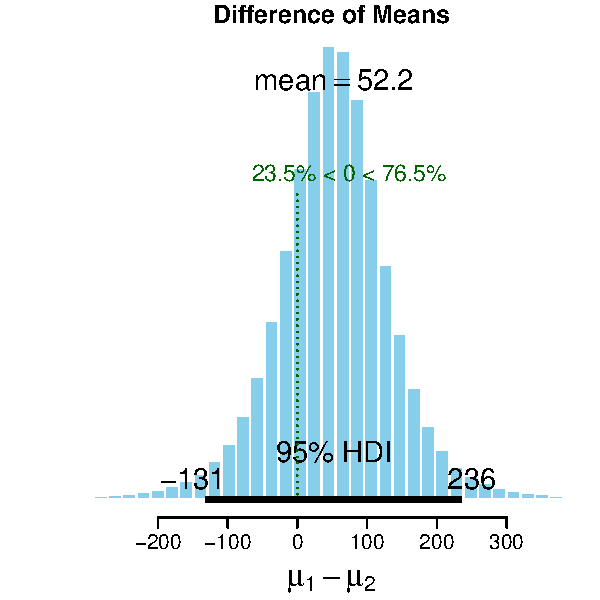
\includegraphics[width=\figwidth]{figures/cropped/djpeg-m-single-uni}
            }\hspace{-.05\textwidth}
            \subfloat[\objdump\\single vs.\ union]{%
                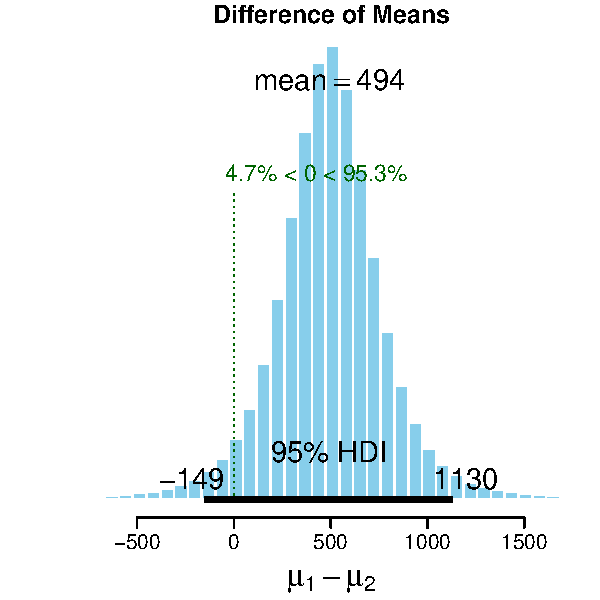
\includegraphics[width=\figwidth]{figures/cropped/objdump-m-single-uni}
            }\hspace{-.05\textwidth}
            \subfloat[\tiffpdf\\multi vs.\ union]{%
                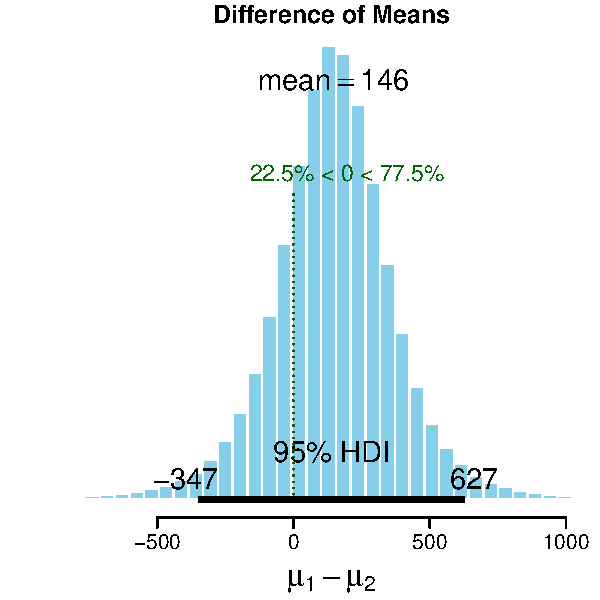
\includegraphics[width=\figwidth]{figures/cropped/tiff2pdf-m-multi-uni}
            }\hspace{-.05\textwidth}
            \subfloat[\listswf\\multi vs.\ union]{%
                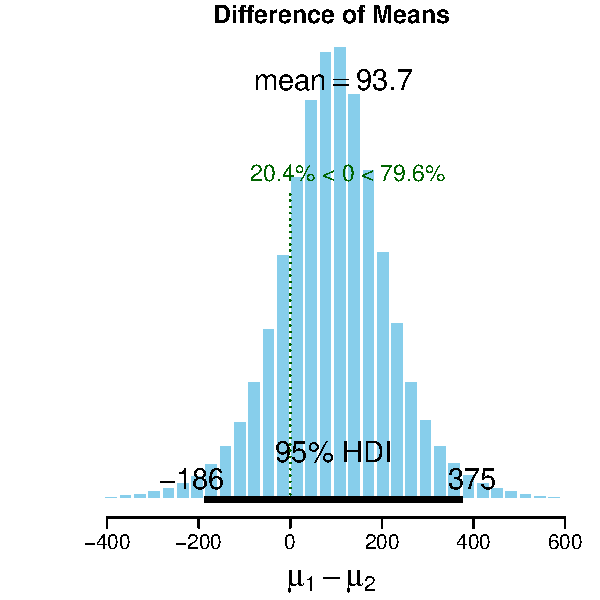
\includegraphics[width=\figwidth]{figures/cropped/ming-m-multi-uni}
            }
        \end{adjustbox}
    \end{figure}
\end{frame}

\subsection{Crash Analysis and Known Vulnerabilities}

\begin{frame}{Unique Crash Analysis}
    \begin{block}{Obtaining unique crashes}
        \begin{enumerate}
            \item{} fuzzers collect unique crashes in folder
            \item{} re-execute SUT with input and run \texttt{exploitable} (stack hash)
            \item{} stack hash and elapsed time for 5 runs in single file
        \end{enumerate}
    \end{block}
    \vspace{\baselineskip}
    \begin{table}
        \begin{tabular}{l c c c c}
            & \textbf{Unique crashes} & \textbf{Vs.\ single} &
\textbf{Vs.\ multi} & \textbf{Vs.\ union} \\
\bottomrule%
\textbf{union} & $75$ & $21$ & $13$ & \\
\hline%
\textbf{multi} & $98$ & $44$ & & $36$ \\
\hline%
\textbf{single} & $63$ & & $9$ & $9$


        \end{tabular}
    \end{table}
\end{frame}

\begin{frame}{Unique Crashes Over Time}
    \renewcommand\figwidth{.32\textwidth}
    \setcounter{subfigure}{0}
    \captionsetup[subfigure]{margin=3pt}
    \begin{figure}
        \subfloat[Cumulative count of unique crashes]{%
            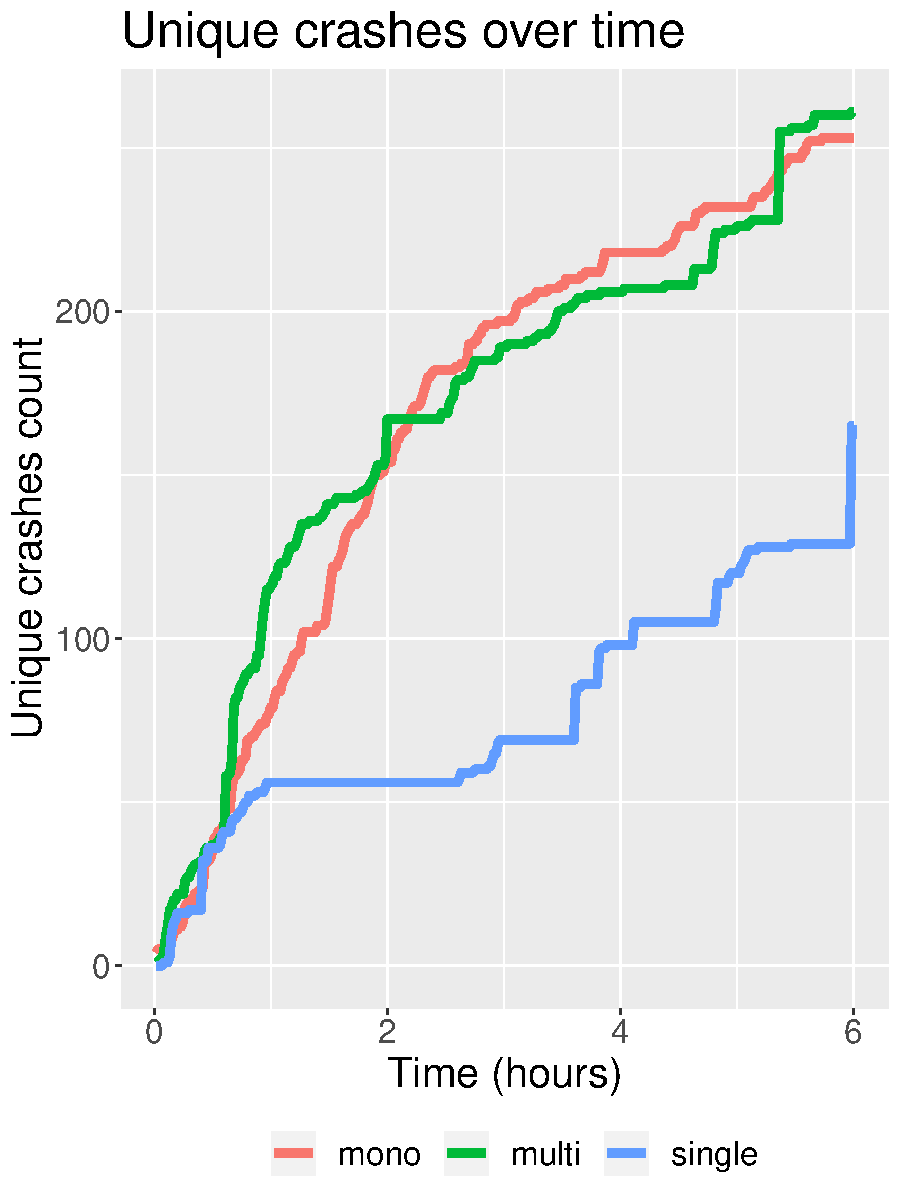
\includegraphics[width=\figwidth]{figures/cropped/crashes-count-all}
        }
        \subfloat[Density of unique crashes]{%
            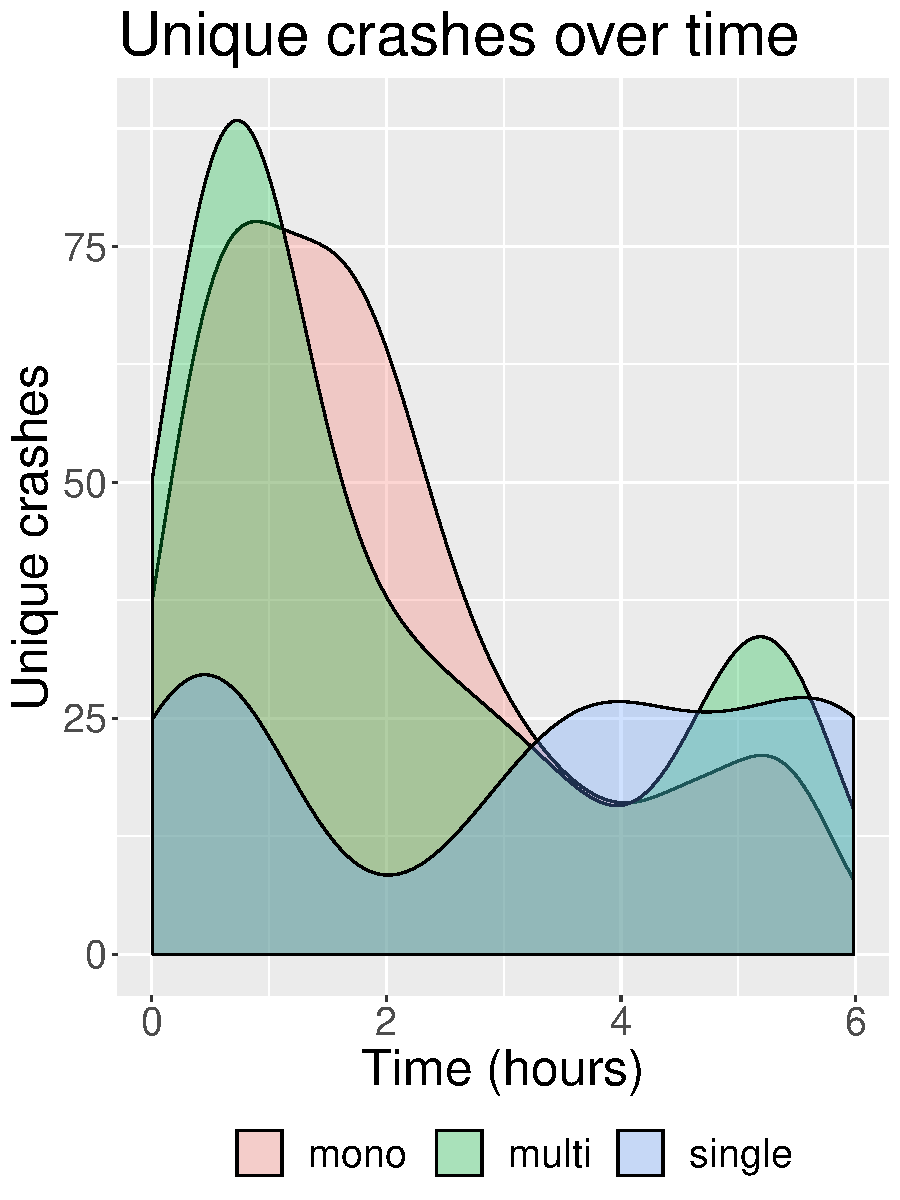
\includegraphics[width=\figwidth]{figures/cropped/crashes-all}
        }
        \subfloat[Uncommon unique crashes]{%
            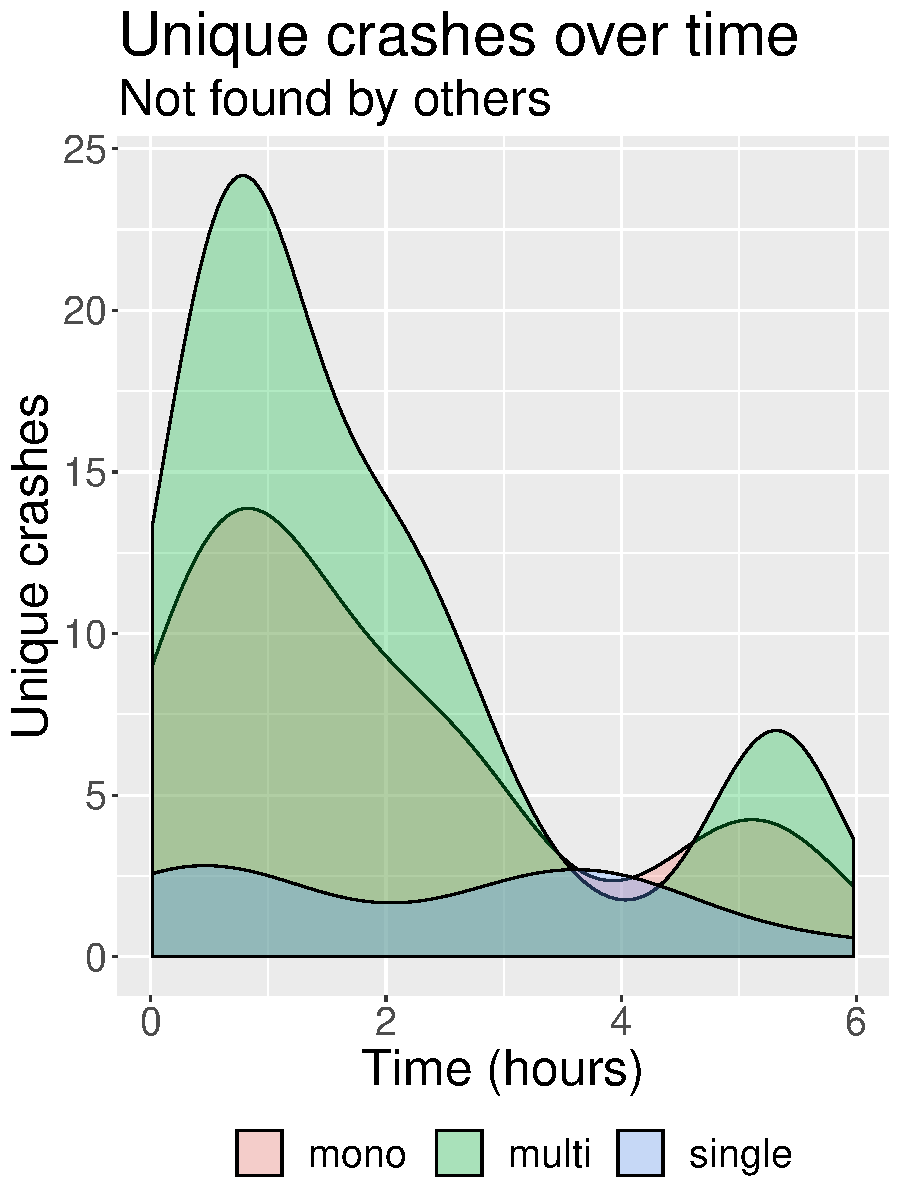
\includegraphics[width=\figwidth]{figures/cropped/crashes-not-intersect}
        }
    \end{figure}
\end{frame}

\begin{frame}{Known Vulnerabilities}
    \begin{columns}
        \begin{column}{.66\textwidth}
            \renewcommand\figwidth{.33\textwidth}
            \vspace{-20pt}
            \begin{figure}
                \subfloat{%
                    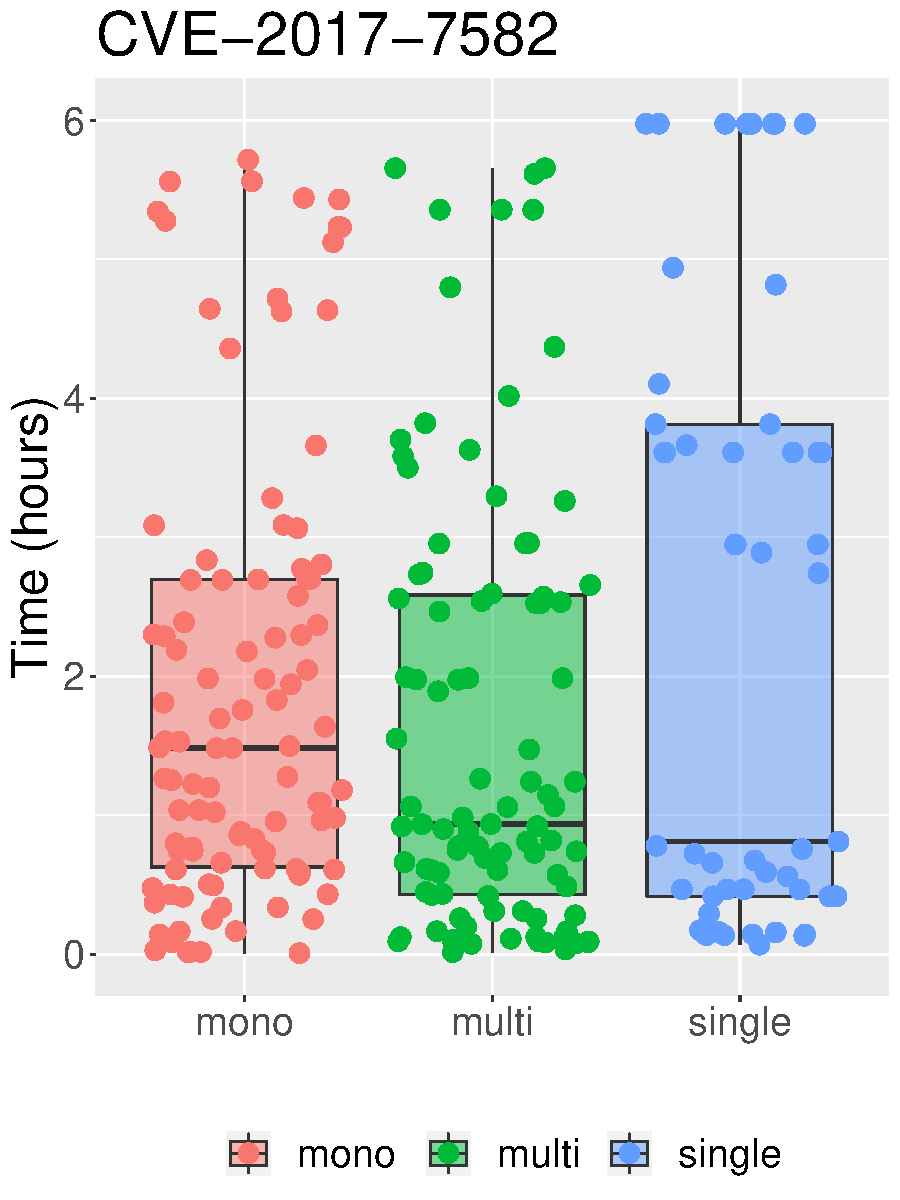
\includegraphics[width=\figwidth]{figures/cropped/cve-2017-7582}
                }
                \subfloat{%
                    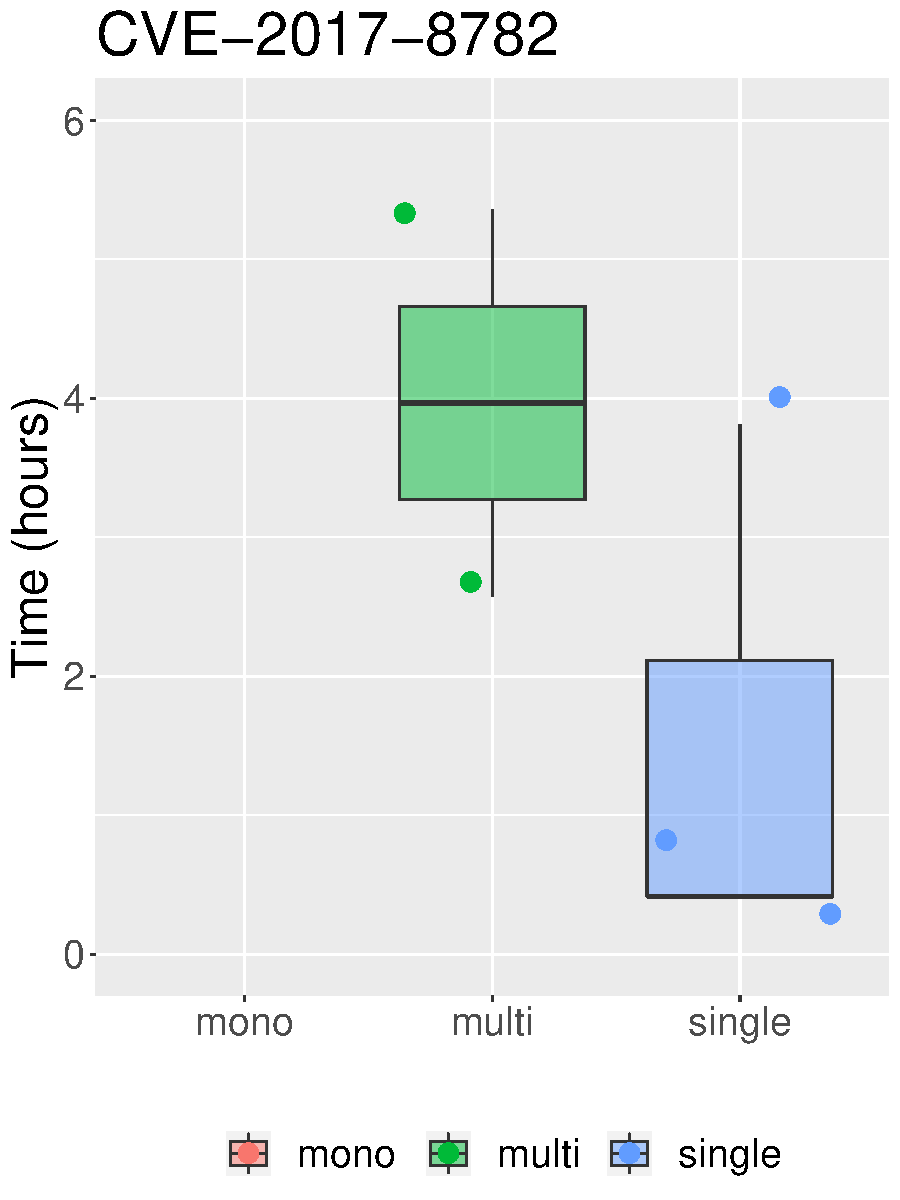
\includegraphics[width=\figwidth]{figures/cropped/cve-2017-8782}
                }
                \subfloat{%
                    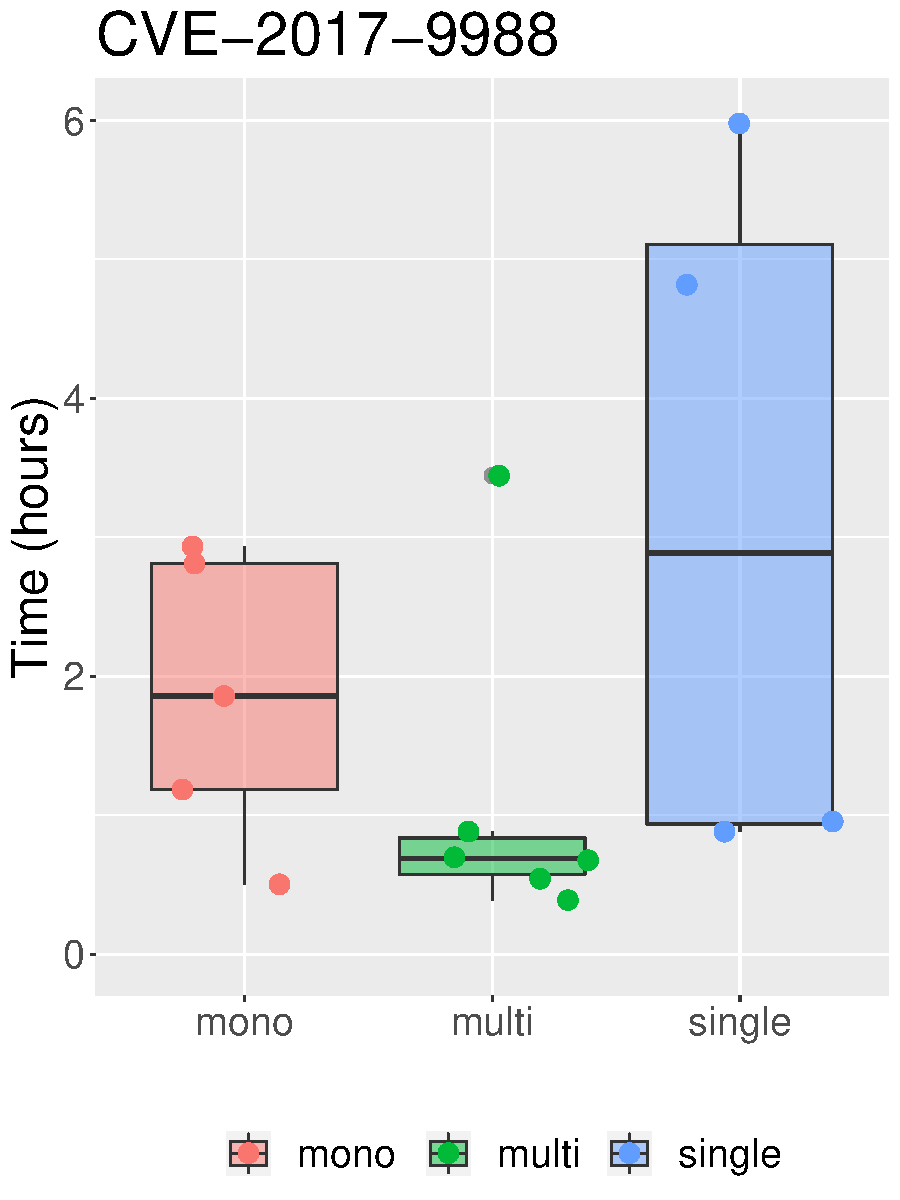
\includegraphics[width=\figwidth]{figures/cropped/cve-2017-9988}
                }
                \vspace{-8pt}
                \subfloat{%
                    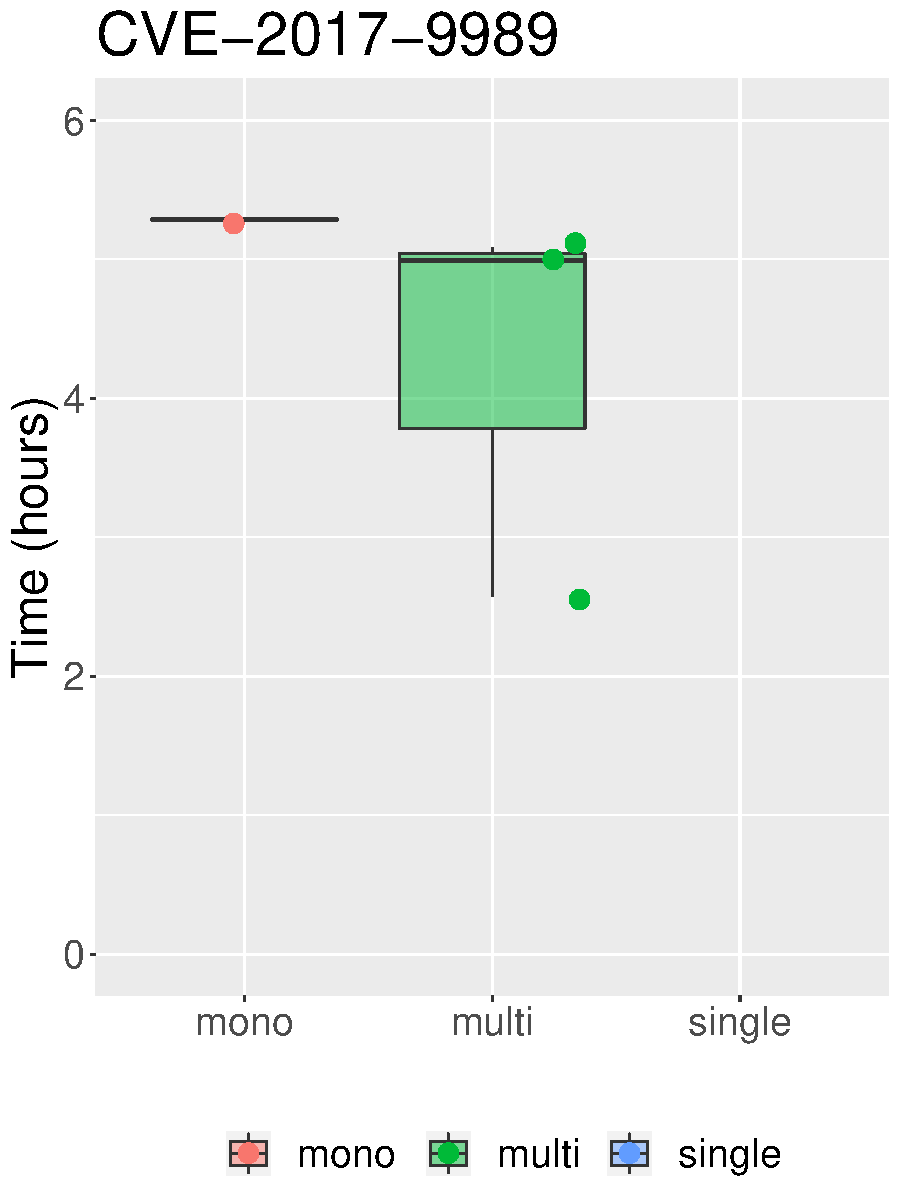
\includegraphics[width=\figwidth]{figures/cropped/cve-2017-9989}
                }
                \subfloat{%
                    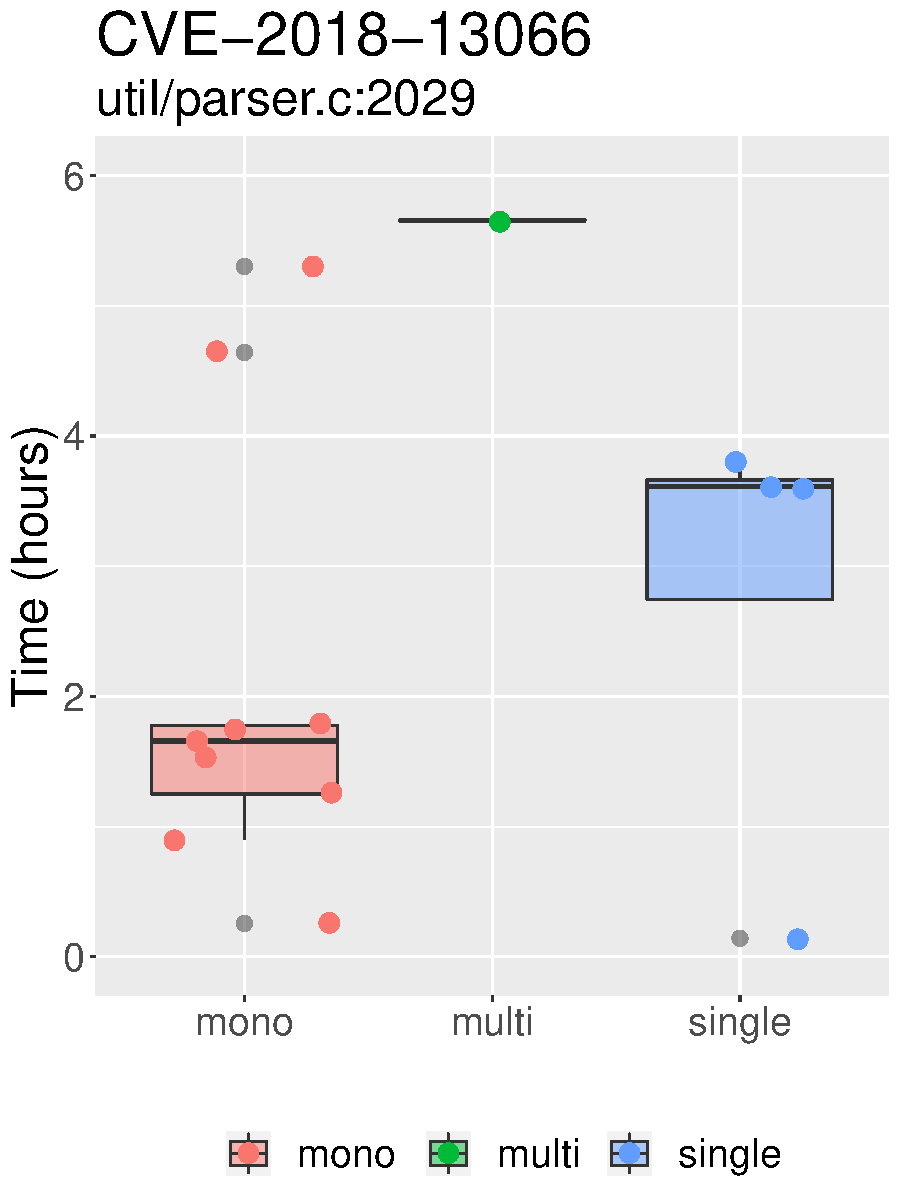
\includegraphics[width=\figwidth]{figures/cropped/cve-2018-13066-parser-2029}
                }
                \subfloat{%
                    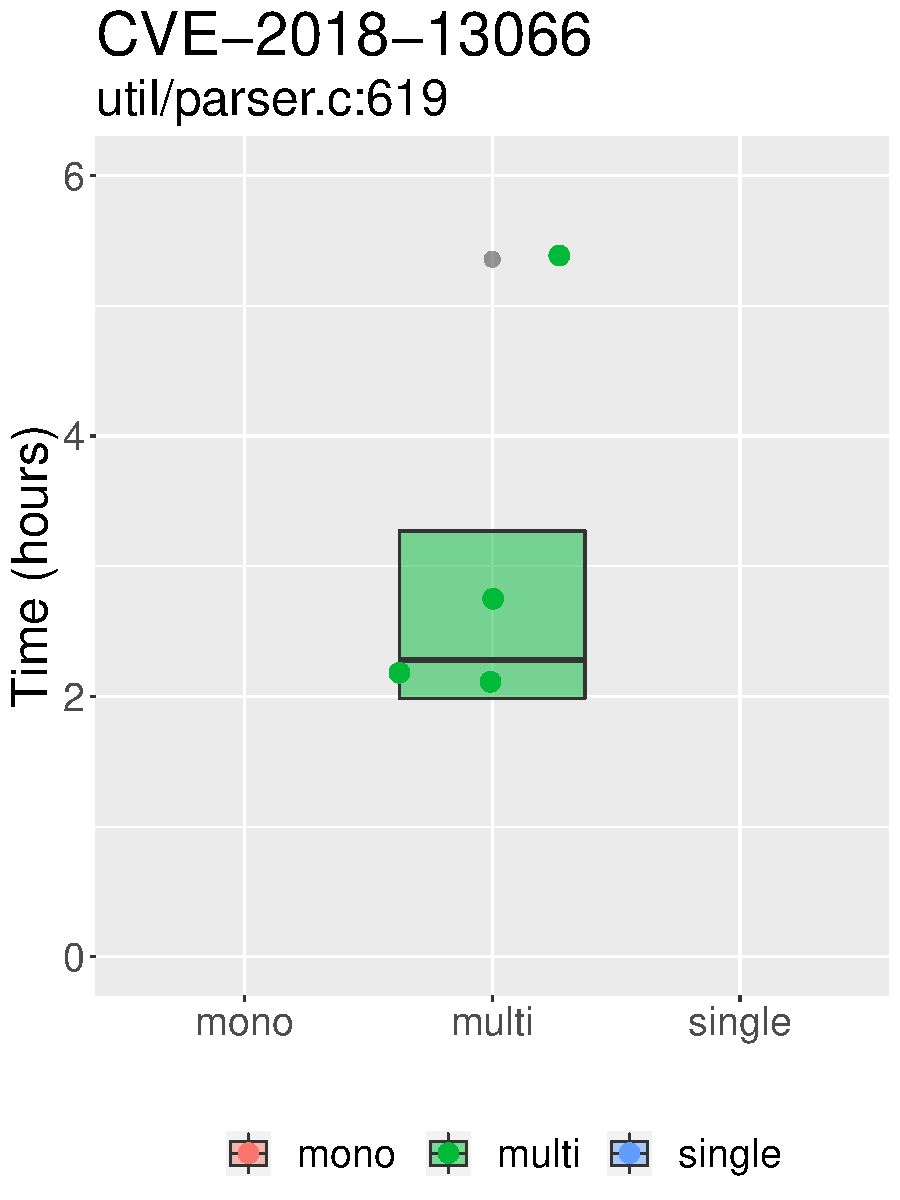
\includegraphics[width=\figwidth]{figures/cropped/cve-2018-13066-parser-619}
                }
            \end{figure}
        \end{column}
        \begin{column}{.33\textwidth}
            \begin{itemize}
                \item{} over 25 bugs,\\6 linked to a CVE
                \item{} multi winners\\finds all CVE\\found by union
                \item{} all but one found earlier than union
                \item{} finds two CVE\\not found by union
            \end{itemize}
        \end{column}
    \end{columns}
\end{frame}

\section{Discussion and Future Work}

\subsection*{Discussion}

\subsection*{Future Work}

\end{document}
